\documentclass{beamer}
\usetheme{Boadilla}
\usepackage[utf8x]{inputenc}
\usepackage{listings}
\usepackage{subfig}
\title{LS IoT Platform}
\subtitle{Piattaforma per il monitoraggio di macchine utensili con integrazione a software ERP Microsoft Dynamics NAV}
\author{Vincenzo Nucci e Matteo Tiberi}
%\author{Matteo Tiberi}
\institute{Università di Camerino}
\date{}
\begin{document}
	
	\begin{frame}
	\centering
	
\includegraphics[scale=0.7]{images/stemma.png}\par
	\usebeamertemplate{title page}
\end{frame}


\begin{frame}
\frametitle{LS IoT Platform}
\begin{itemize}
	\item Espone servizi REST per letture di sensori
	\begin{itemize}
		\item Ultima lettura di un sensore
		\item Letture di una certa settimana
		\item Letture di un certo mese
		\item Letture di determinati campi dei sensori
	\end{itemize}
	\item Servizio di sottoscrizione con notifiche PUSH
	\begin{itemize}
		\item Debolmente accoppiato grazie ad Apache ActiveMQ
	\end{itemize}
	\item Integra il servizio di sottoscrizione con Dynamics NAV
	\begin{itemize}
		\item Utilizzo dei web services SOAP offerti da NAV
	\end{itemize}
	\item Indipendente da sorgenti dati e formato dei dati
	\begin{itemize}
		\item Grazie a classi astratte, interfacce e Apache Avro
	\end{itemize}
	\item Interfaccia web
	\begin{itemize}
		\item Pagina per la registrazione delle applicazioni
		\item Pagina per la gestione delle richieste
		\item Pagina per la gestione dei servizi attivi per gli utenti
	\end{itemize}
\end{itemize}
\end{frame}

\begin{frame}
\frametitle{Architettura piattaforma}
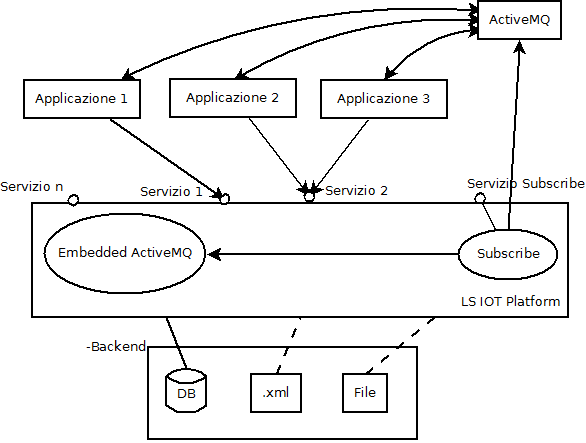
\includegraphics[width=0.9\textwidth]{images/architettura_piattaforma.png}
\end{frame}

\begin{frame}
\frametitle{Struttura tabelle backend}
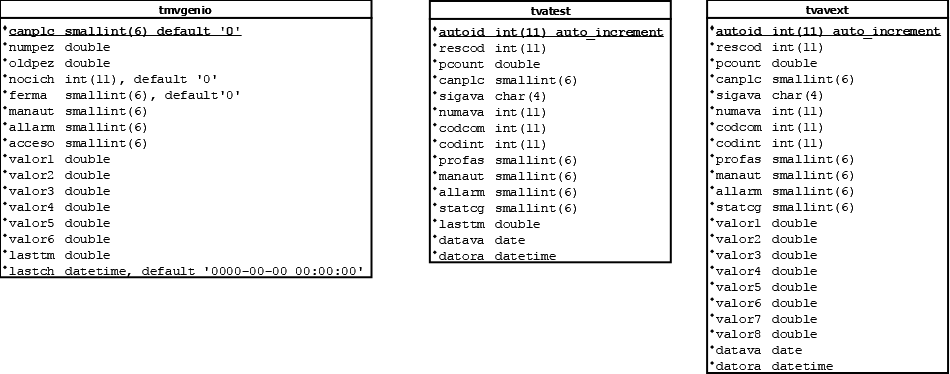
\includegraphics[width=1\textwidth]{images/tabelle-backend.png}
\end{frame}

\begin{frame}
\frametitle{Pagina web richiesta token}
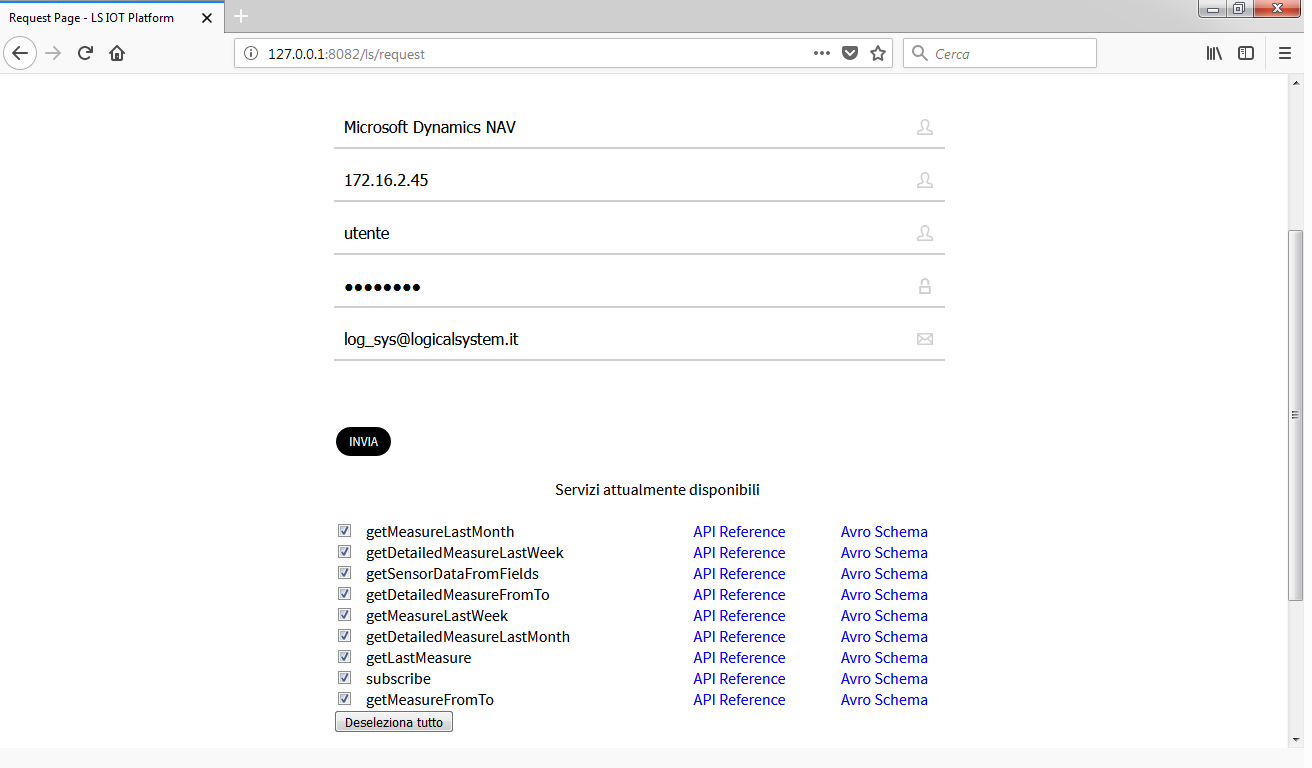
\includegraphics[width=1\textwidth]{images/RequestPagePlatform.png}
\end{frame}

\begin{frame}
\frametitle{Gestione delle richieste nel database}
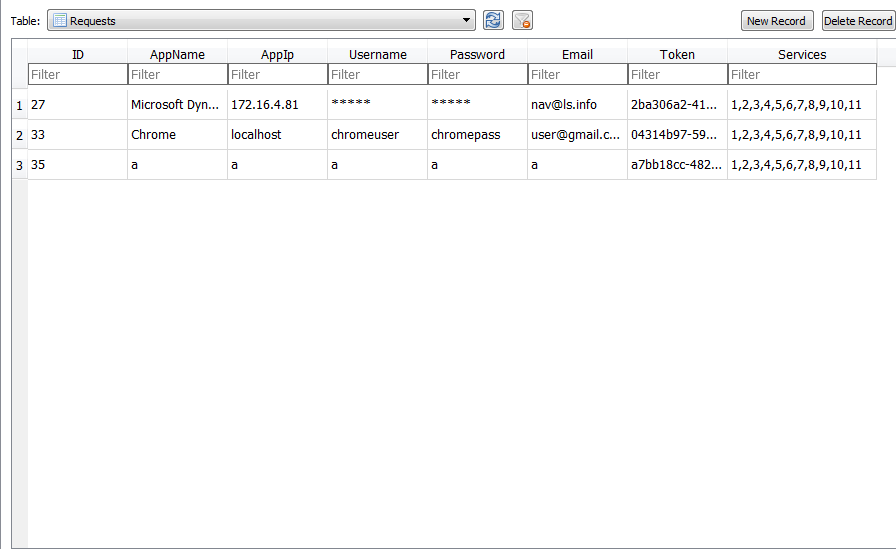
\includegraphics[width=1\textwidth]{images/DBPlatform2.png}
\end{frame}

\begin{frame}
\frametitle{Pagina web gestione delle richieste}
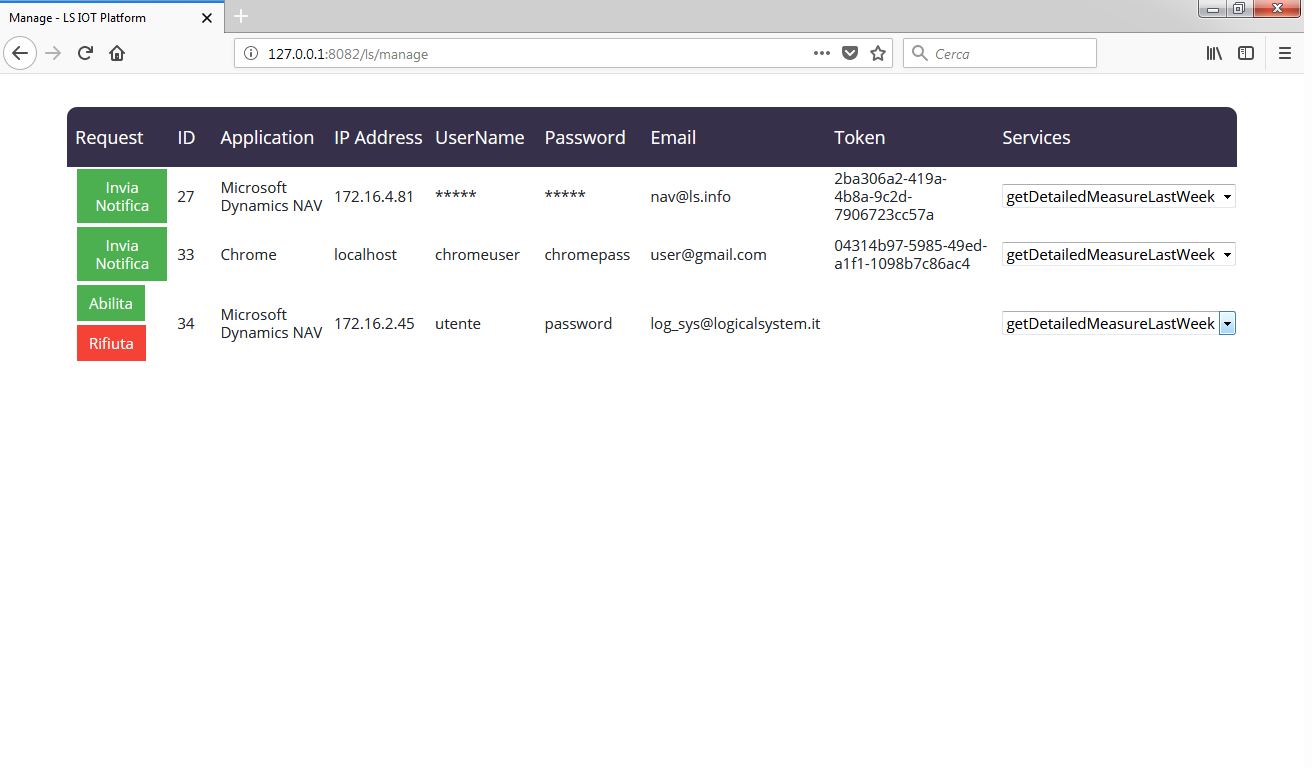
\includegraphics[width=1\textwidth]{images/managePagePlatform.png}
\end{frame}

\begin{frame}
\frametitle{Sottoscrizioni database}
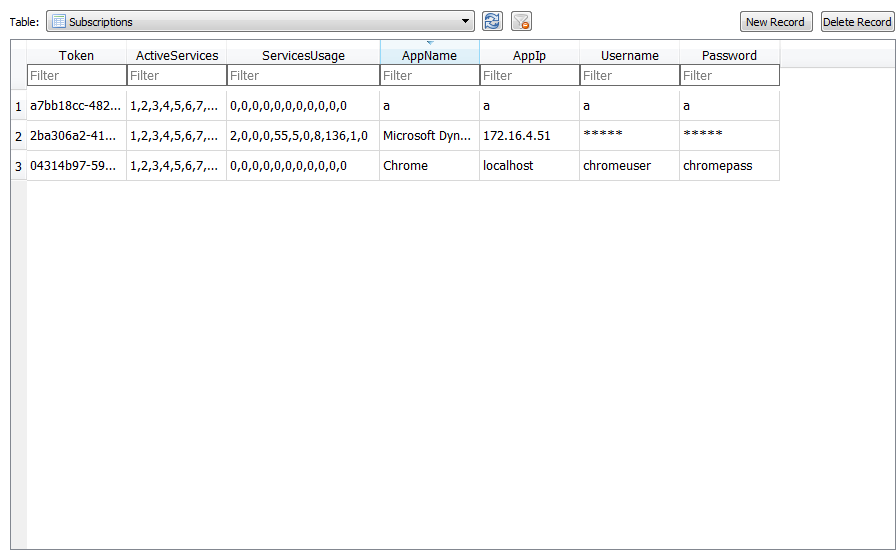
\includegraphics[width=1\textwidth]{images/DBPlatform3.png}
\end{frame}

\begin{frame}
\frametitle{Pagina web gestione dei servizi utenti}
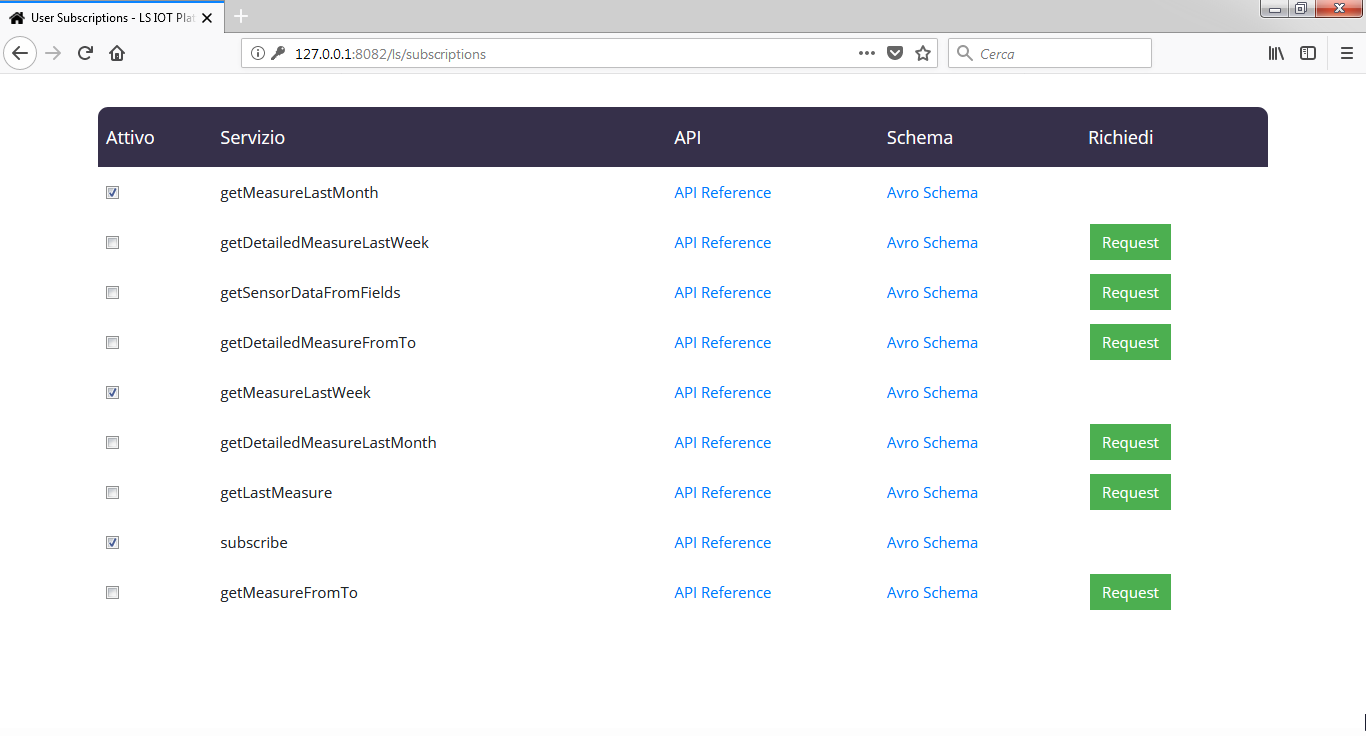
\includegraphics[width=1\textwidth]{images/UserSubscriptionsPlatform.png}
\end{frame}

\begin{frame}
\frametitle{Esempio di un servizio}
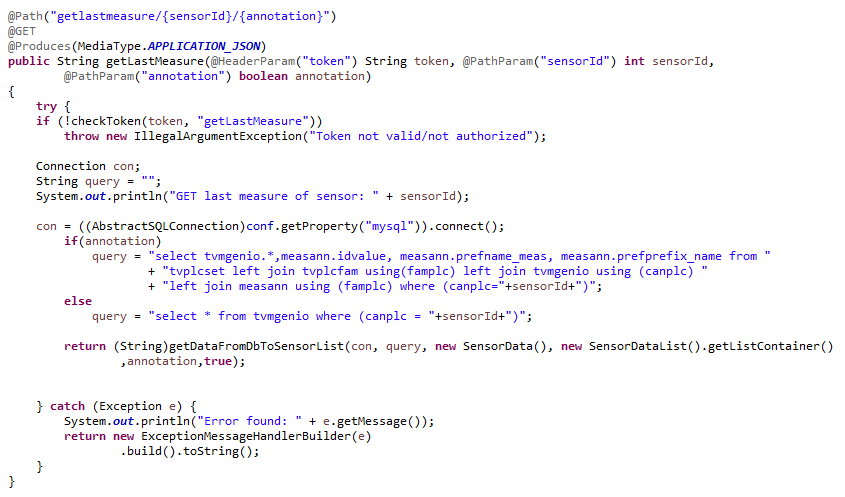
\includegraphics[width=1\textwidth]{images/getlastmeasure.png}
\end{frame}

\begin{frame}
\frametitle{Valori di ritorno di getlastmeasure}
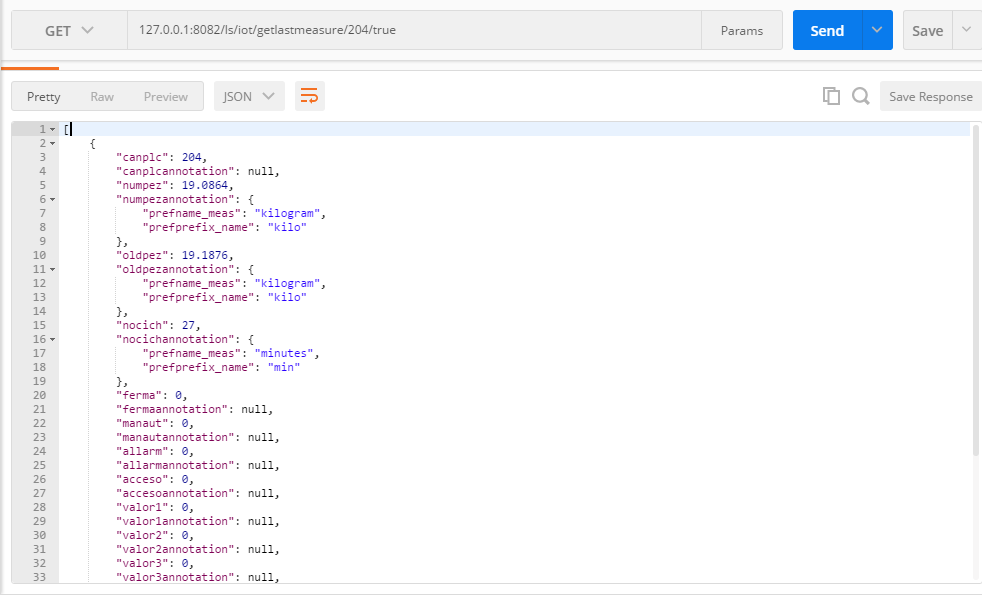
\includegraphics[width=1\textwidth]{images/Postman1.png}
\end{frame}

\begin{frame}
\frametitle{Pagina catalogo Smart Object}
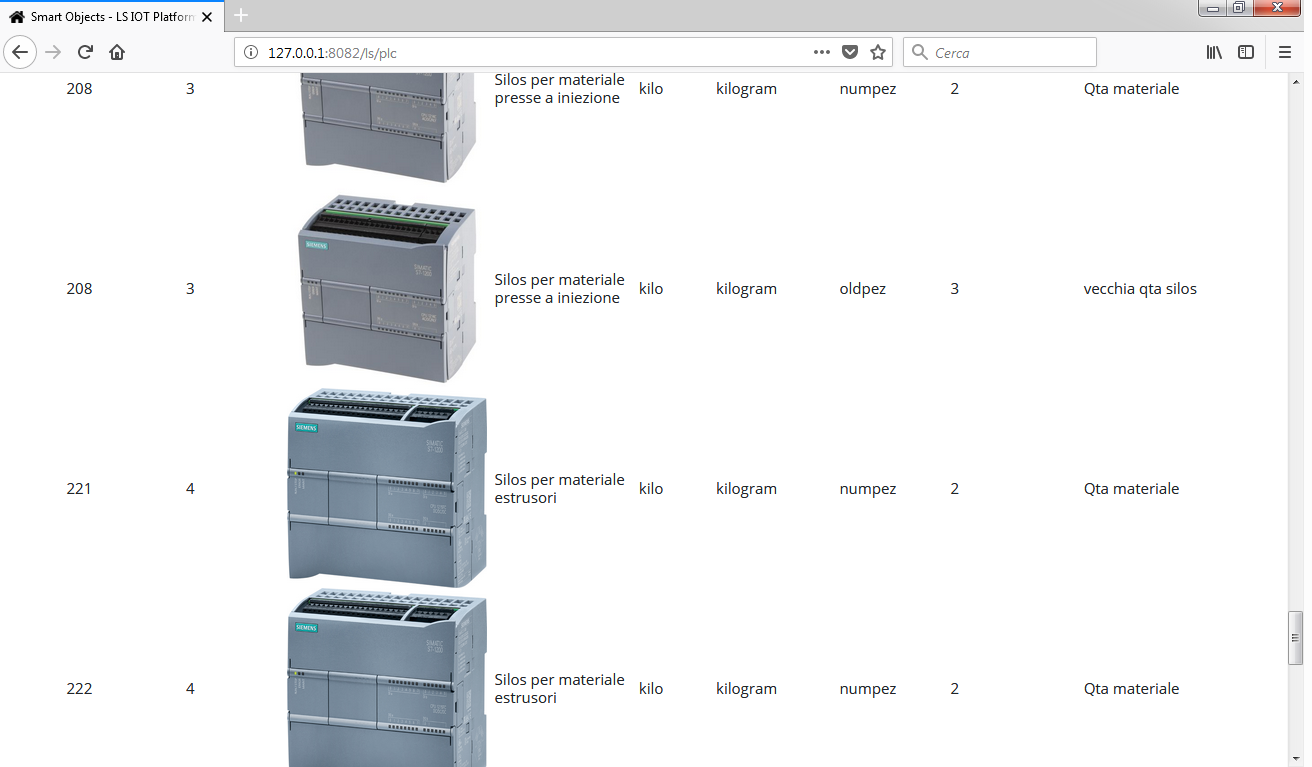
\includegraphics[width=1\textwidth]{images/SmartObjectsPlatform.png}
\end{frame}

\begin{frame}
\frametitle{Subscribe Rule}
\begin{itemize}
\item Messaggio JSON che il servizio di sottoscrizione si aspetta di ricevere
\item L'utente specifica la condizione
\begin{itemize}
\item Nome e IP applicazione
\item Coda o topic di ActiveMQ
\item Rule Record
\begin{itemize}
\item Nome tabella da interrogare
\item Lista dei campi dei quali monitorarne i cambiamenti
\item Espressione CRON
\item Clausola where

\end{itemize}
\end{itemize}
\end{itemize}
\end{frame}

\begin{frame}
\frametitle{Clausola where}
\begin{itemize}
\item Condition
\begin{itemize}
\item insieme di oggetti Avro annidati
\end{itemize}
\item Formula
\begin{itemize}
\item Semplice stringa (per NAV)
\end{itemize}
\end{itemize}
\end{frame}

\begin{frame}
\frametitle{Albero della condition}
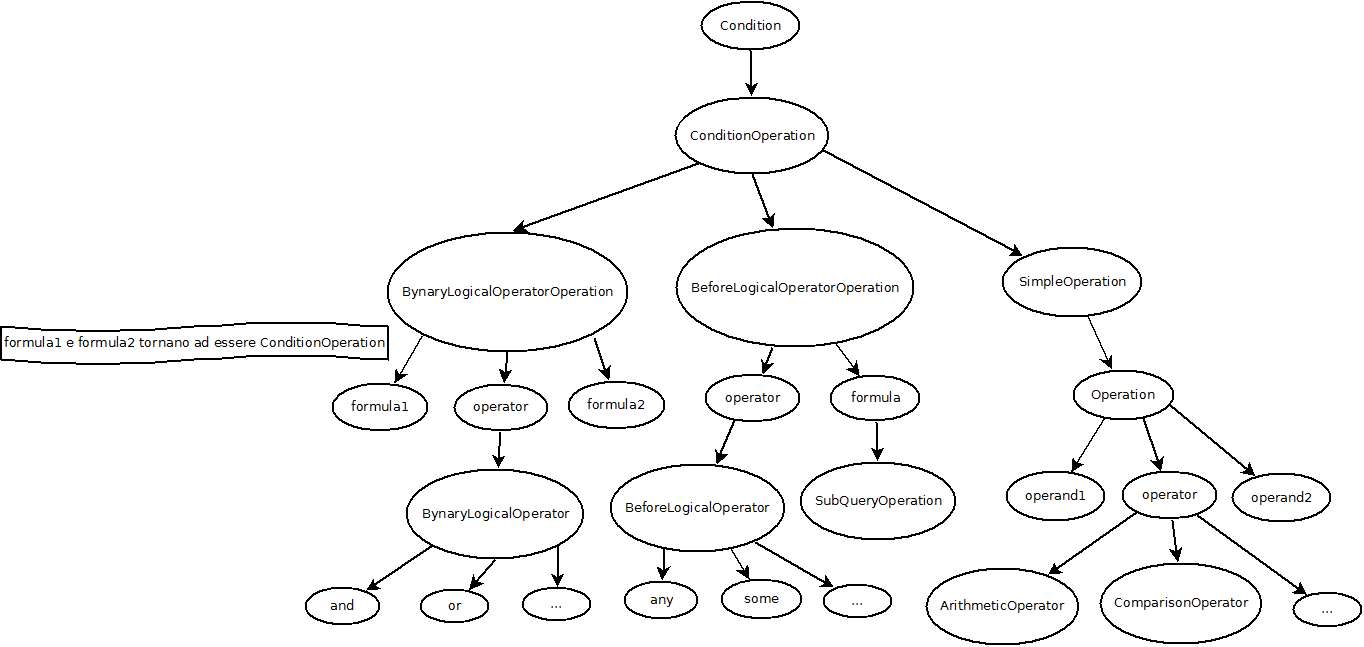
\includegraphics[width=1\textwidth]{images/strutturaquerytree.png}
\end{frame}

\begin{frame}
\frametitle{Subscribe Rule di una applicazione}
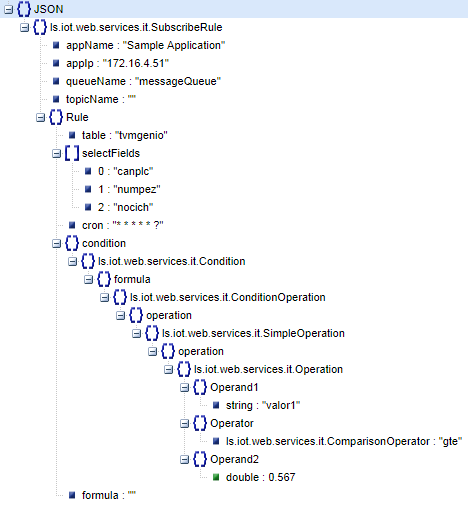
\includegraphics[width=0.6\textwidth]{images/subscribe-json-1.png}
\end{frame}

\begin{frame}
\frametitle{Schema Avro Subscribe Rule di una applicazione}
\begin{figure}%
	\centering
	\subfloat{{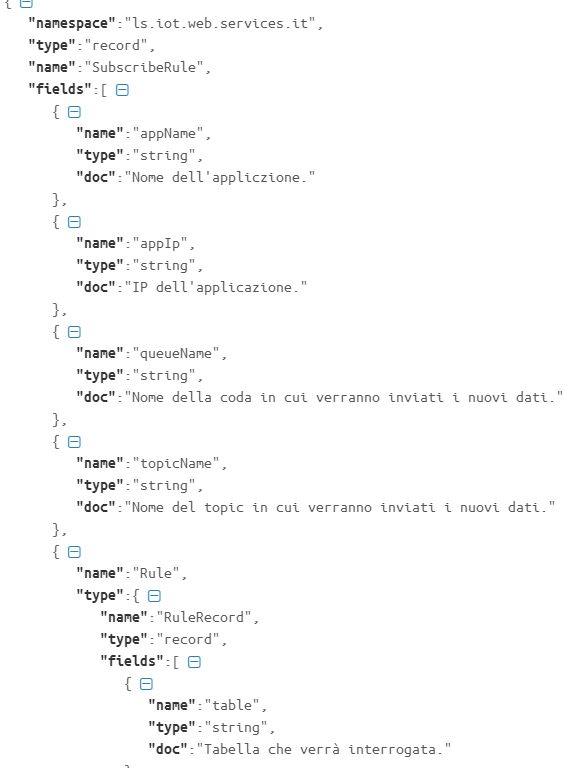
\includegraphics[width=5cm]{images/subscribe-rule-1.png} }}%
	\qquad
	\subfloat{{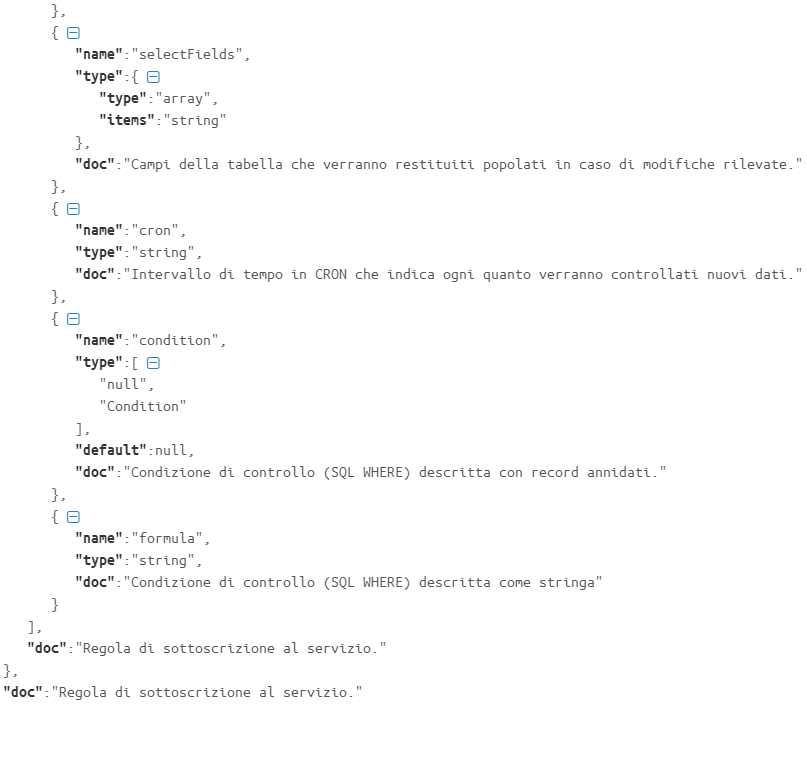
\includegraphics[width=5cm]{images/subscribe-rule-2.png} }}%
	%
	%
\end{figure}
\end{frame}

\begin{frame}
\frametitle{Gestione delle regole nel database}
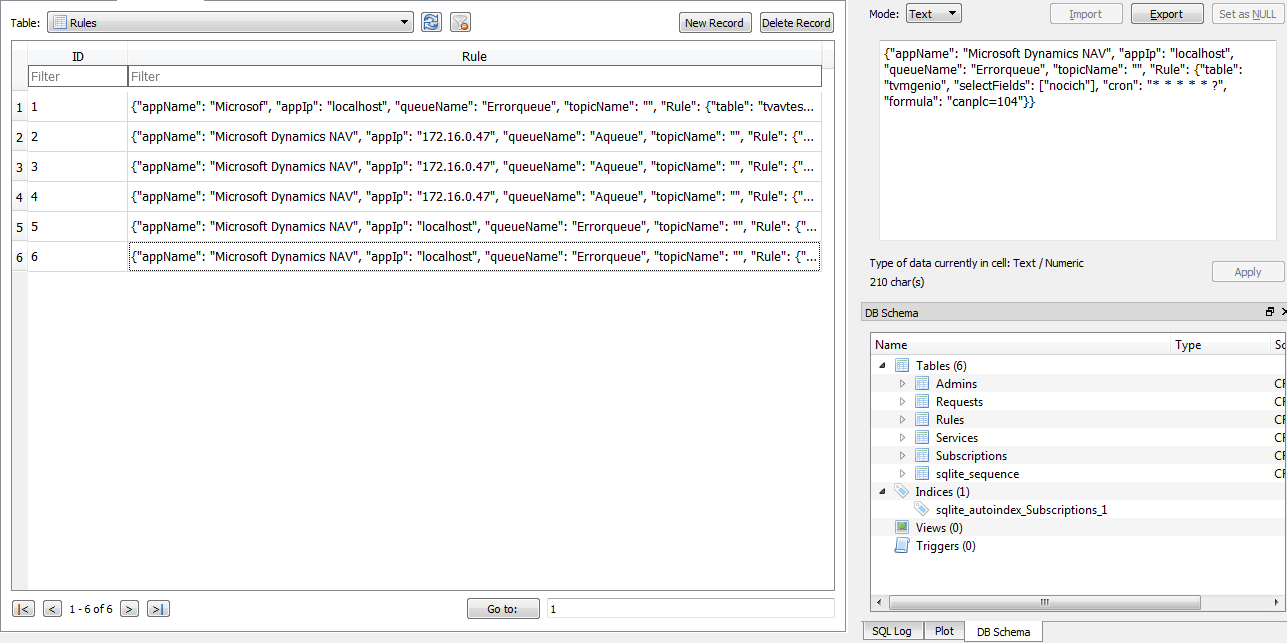
\includegraphics[width=1\textwidth]{images/DBPlatform1.png}
\end{frame}

\begin{frame}
\frametitle{Schema JSON Subscribe Rule di NAV}
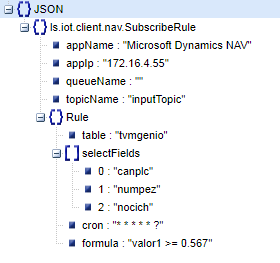
\includegraphics[width=0.6\textwidth]{images/subscribe-json-2.png}
\end{frame}

\begin{frame}
\frametitle{Class Diagram SubscribeRuleInterface}
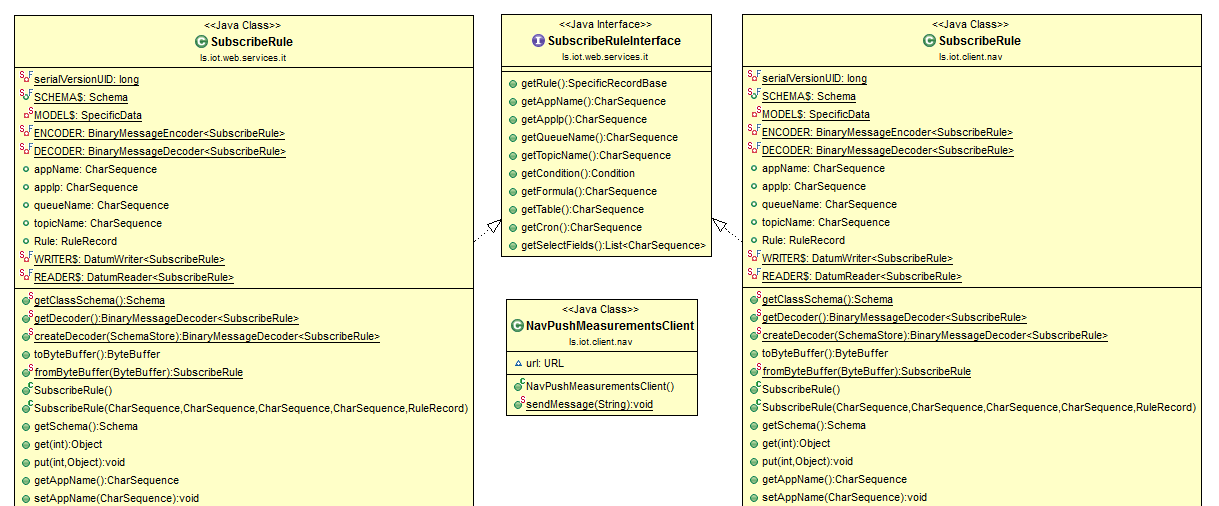
\includegraphics[width=1\textwidth]{images/figura10.png}
\end{frame}

\begin{frame}
\frametitle{Class Diagram RetrievedDataInterface 1}
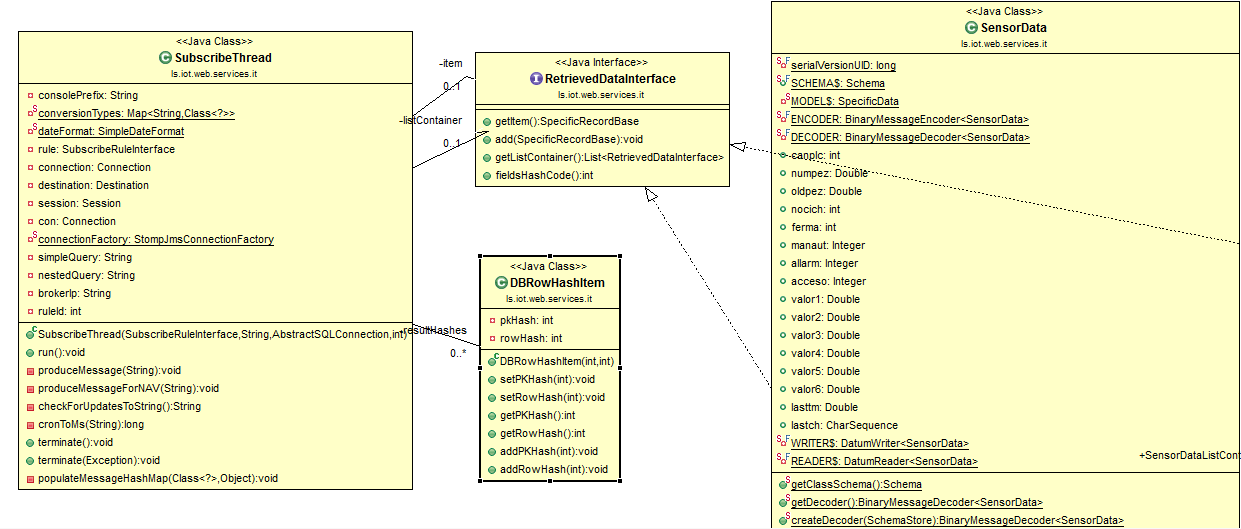
\includegraphics[width=1\textwidth]{images/ClassDiagram2.png}
\end{frame}

\begin{frame}
\frametitle{Class Diagram RetrievedDataInterface 2}
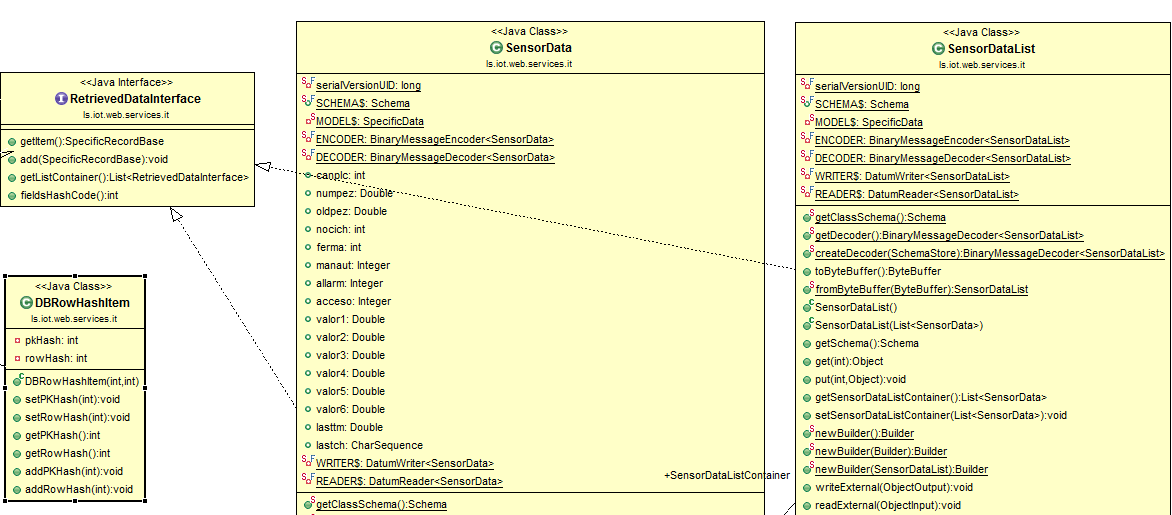
\includegraphics[width=1\textwidth]{images/ClassDiagram1.png}
\end{frame}

\begin{frame}
\frametitle{Schema Avro SensorData}
\begin{figure}%
	\centering
	\subfloat{{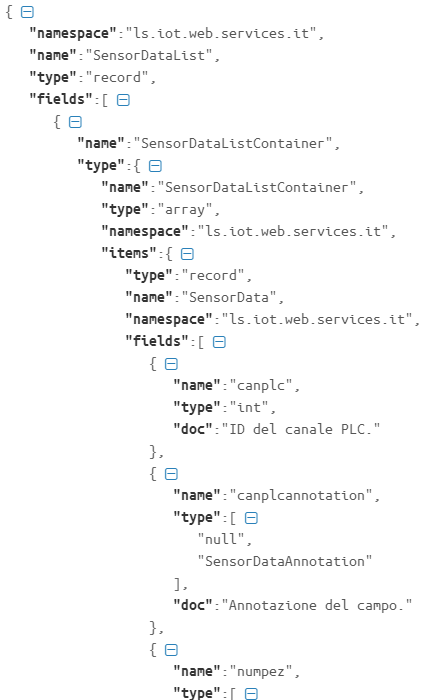
\includegraphics[width=5cm]{images/sensordata1.png} }}%
	\qquad
	\subfloat{{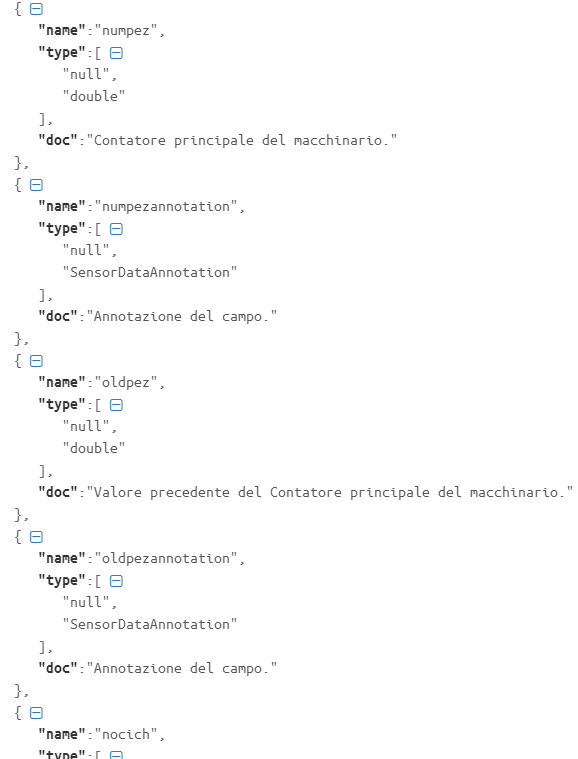
\includegraphics[width=5cm]{images/sensordata2.png} }}%
	%
	%
\end{figure}
\end{frame}

\begin{frame}
\frametitle{Schema Avro SensorDataAnnotation}
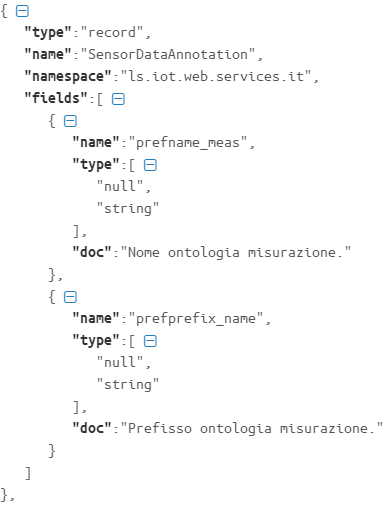
\includegraphics[width=0.6\textwidth]{images/sensordataannotation.png}
\end{frame}

\begin{frame}
\frametitle{Estratto di getDataFromDbToSensorList}
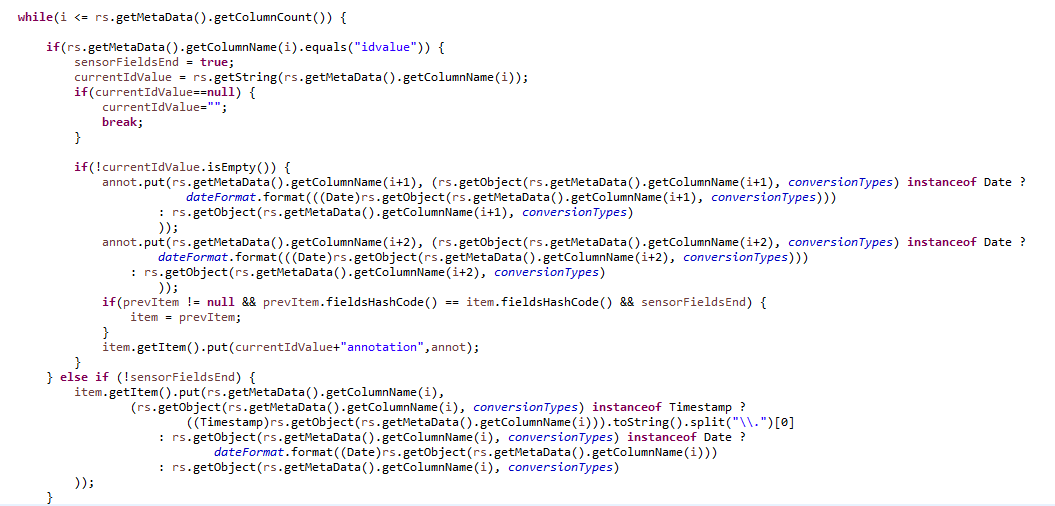
\includegraphics[width=1\textwidth]{images/popolamento-json.png}
\end{frame}

\begin{frame}
\frametitle{Class Diagram AbstractConnection}
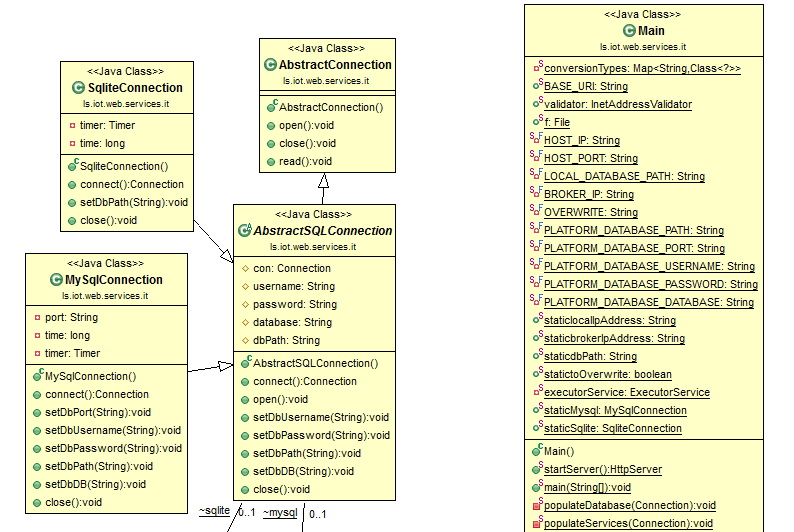
\includegraphics[width=1\textwidth]{images/main.png}
\end{frame}

%-------------------------inizio client-----------------------------
\begin{frame}
\frametitle{Client per la piattaforma}
\begin{itemize}
\item Sviluppato su Microsoft Dynamics NAV nonostante diverse lacune dell'ambiente
\begin{itemize}
\item Mancata possibilità di consumo diretto di servizi REST
\item Mancata possibilità di gestione del formato JSON
\item Difficoltà nell'interazione con software esterni non Microsoft
\end{itemize}
\item Risoluzione tramite sviluppo di un client C\#
\begin{itemize}
\item Con chiamata dei servizi REST, serializzazione e deserializzazione del JSON
\item In conformità con le classi della piattaforma tramite Apache Avro
\item Integrato poi in NAV tramite dll 
\end{itemize}
\item Sviluppo di un "setup" per impostare le chiamate ai servizi su NAV
\begin{itemize}
\item Svolto mediante 2 approcci (PLC e Machine Center)
\item Con trattamento dei dati per l'ambiente Navision
\item Evitando di prendere valori già inseriti o errati
\end{itemize}

\item Interazione con il servizio di sottoscrizione nell'ambiente NAV
\begin{itemize}
\item Tramite esternazione di una codeunit come web service SOAP
\end{itemize}
\end{itemize}
\end{frame}
\begin{frame}
\frametitle{Client NAV}
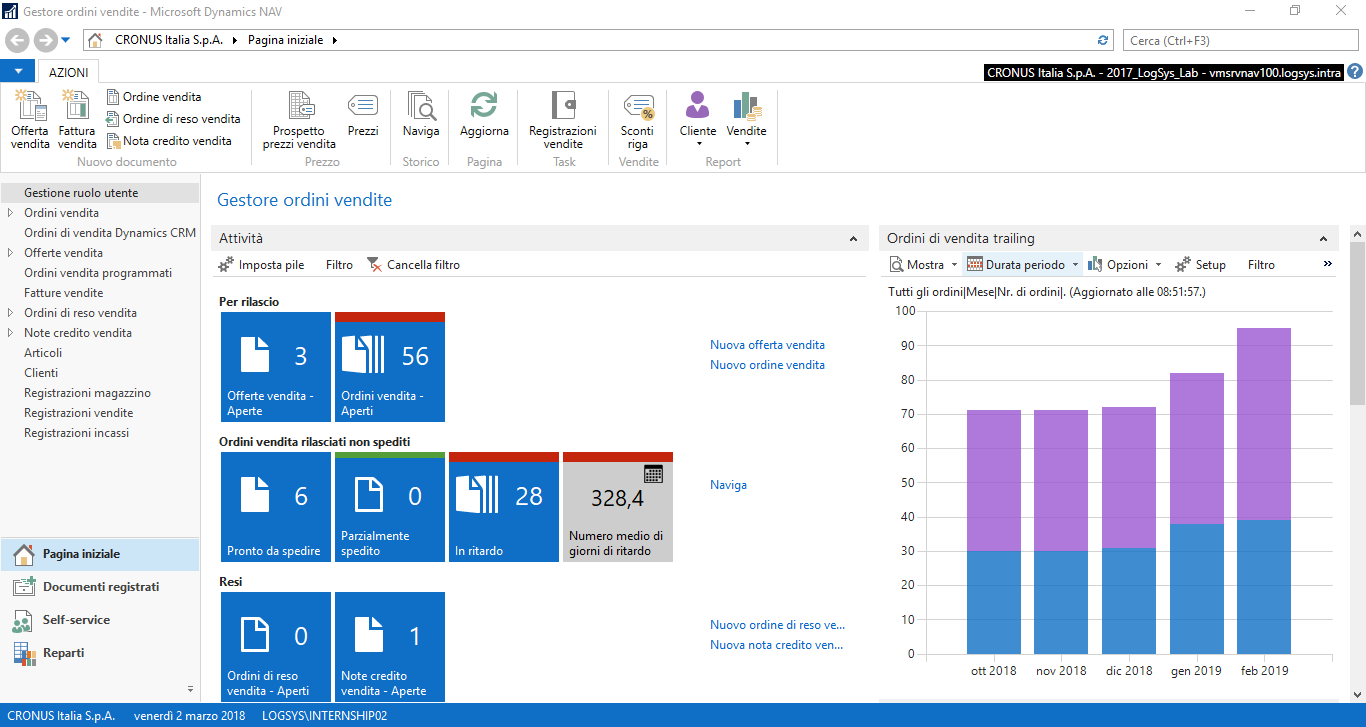
\includegraphics[width=1\textwidth]{images/NAVClient.png}
\end{frame}

\begin{frame}
\frametitle{Class Diagram Client 1}
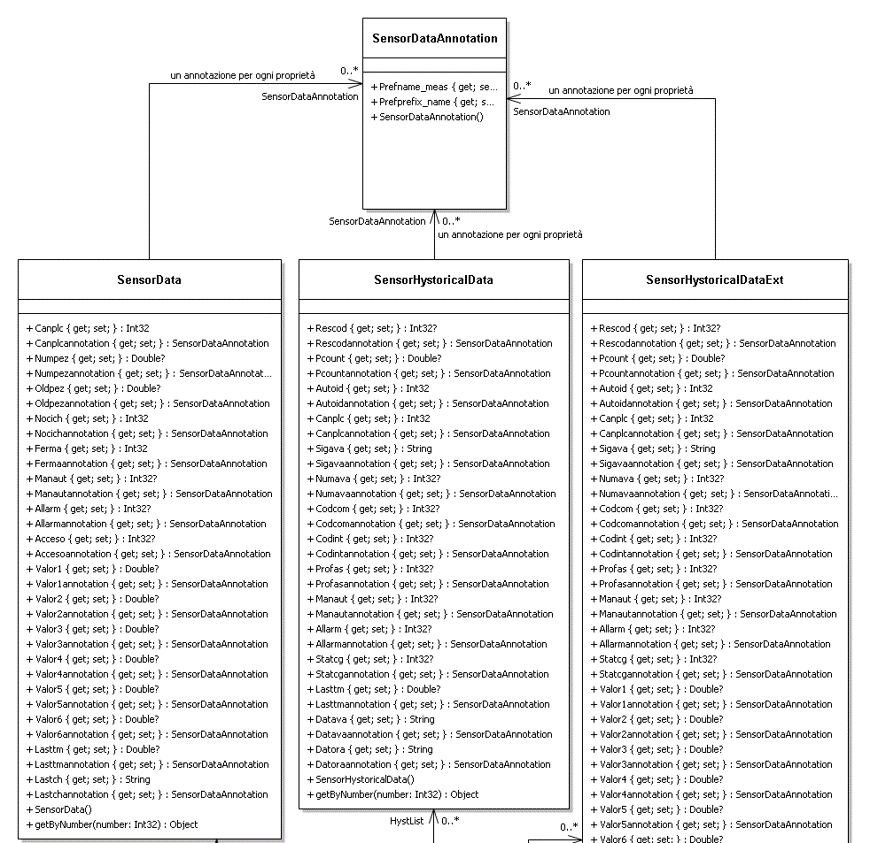
\includegraphics[width=0.6\textwidth]{images/ClassDiagramParte1.png}
\end{frame}

\begin{frame}
\frametitle{Class Diagram Client 2}
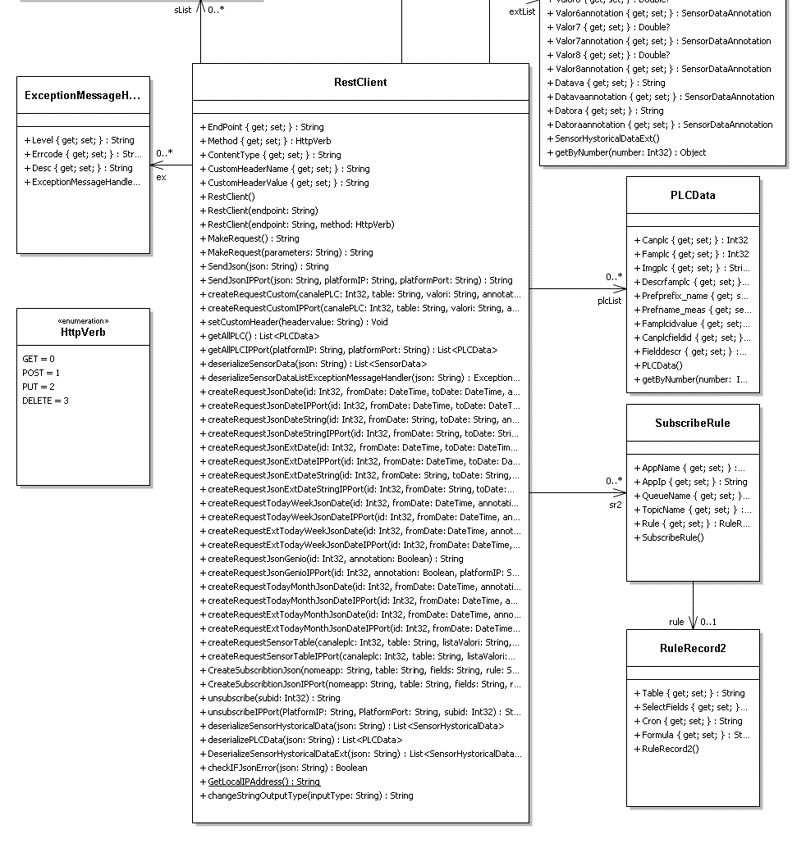
\includegraphics[width=0.6\textwidth]{images/ClassDiagramParte2.png}
\end{frame}

\begin{frame}
\frametitle{Ambiente di sviluppo (C/SIDE) NAV}
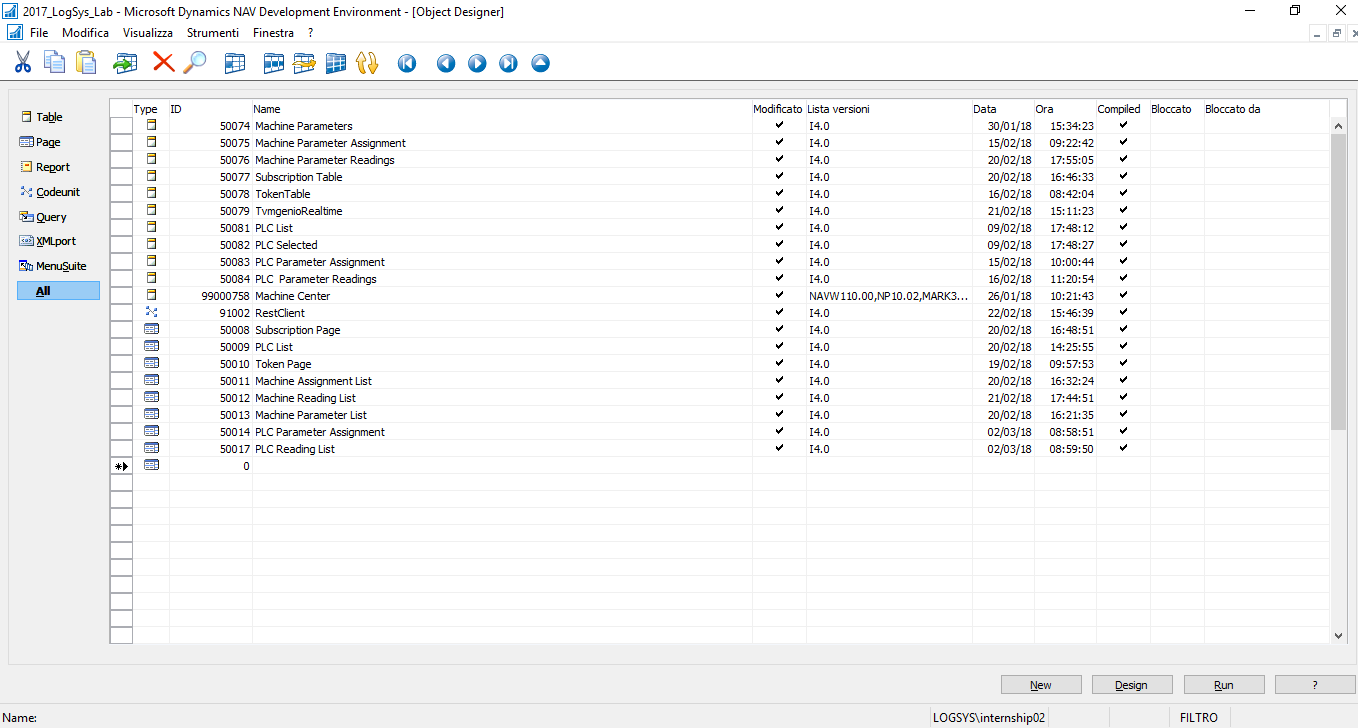
\includegraphics[width=1\textwidth]{images/NAVDevelopmentEnvironment.png}
\end{frame}


\begin{frame}
\frametitle{Lista delle funzioni della codeunit}
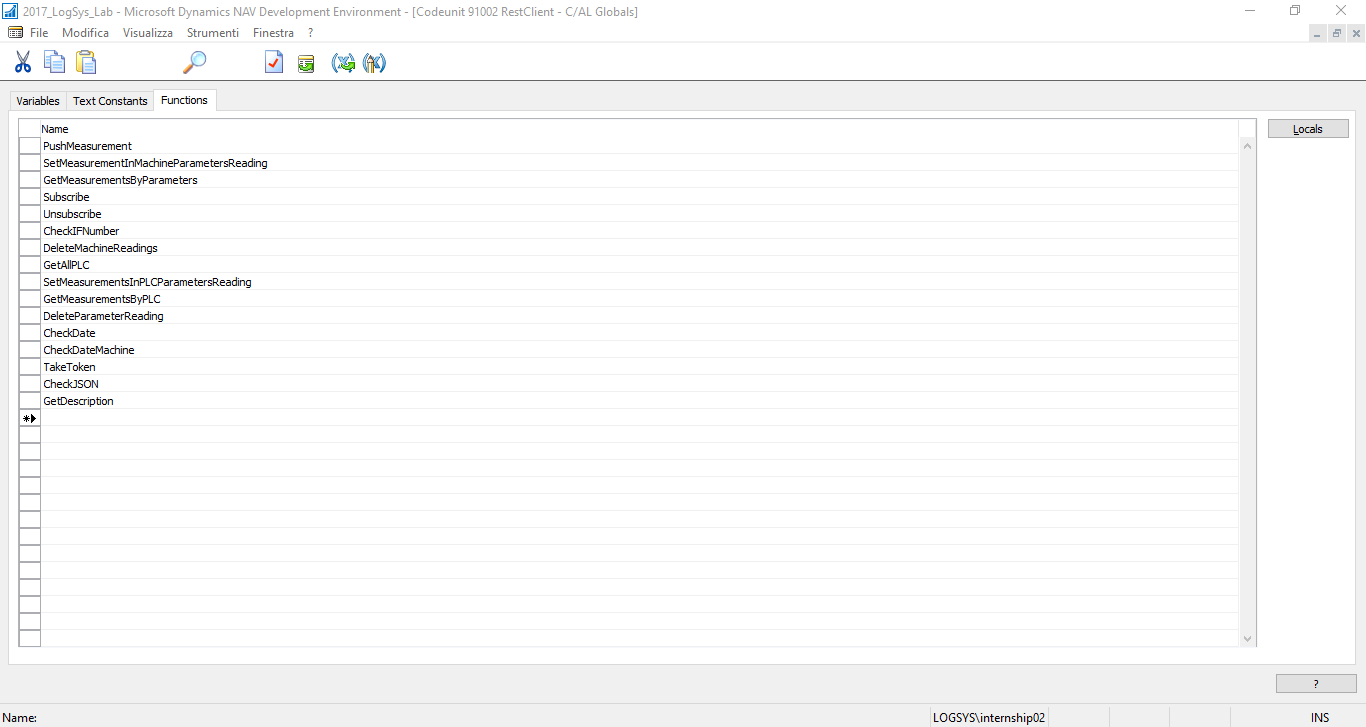
\includegraphics[width=1\textwidth]{images/NAVFunctionList.png}
\end{frame}


\begin{frame}
\frametitle{Lista PLC}
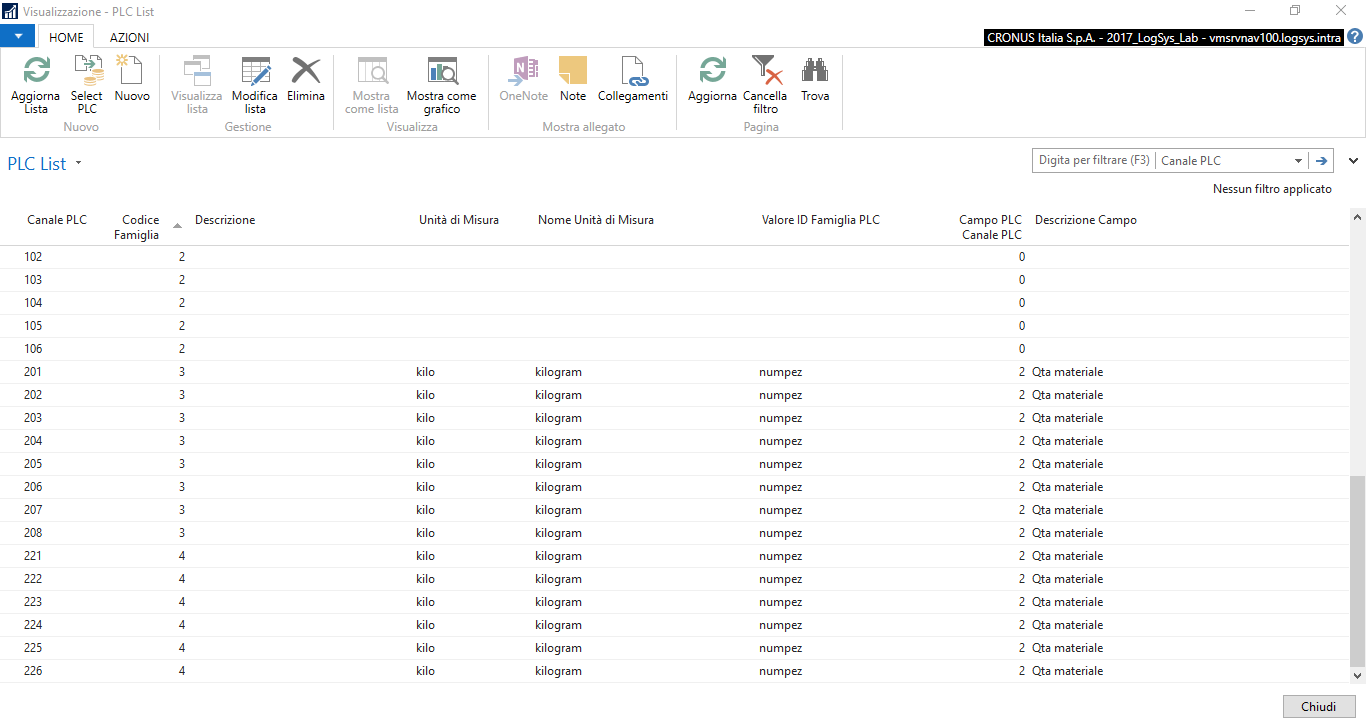
\includegraphics[width=1\textwidth]{images/PLCList.png}
\end{frame}

\begin{frame}
\frametitle{PLC Assignment List}
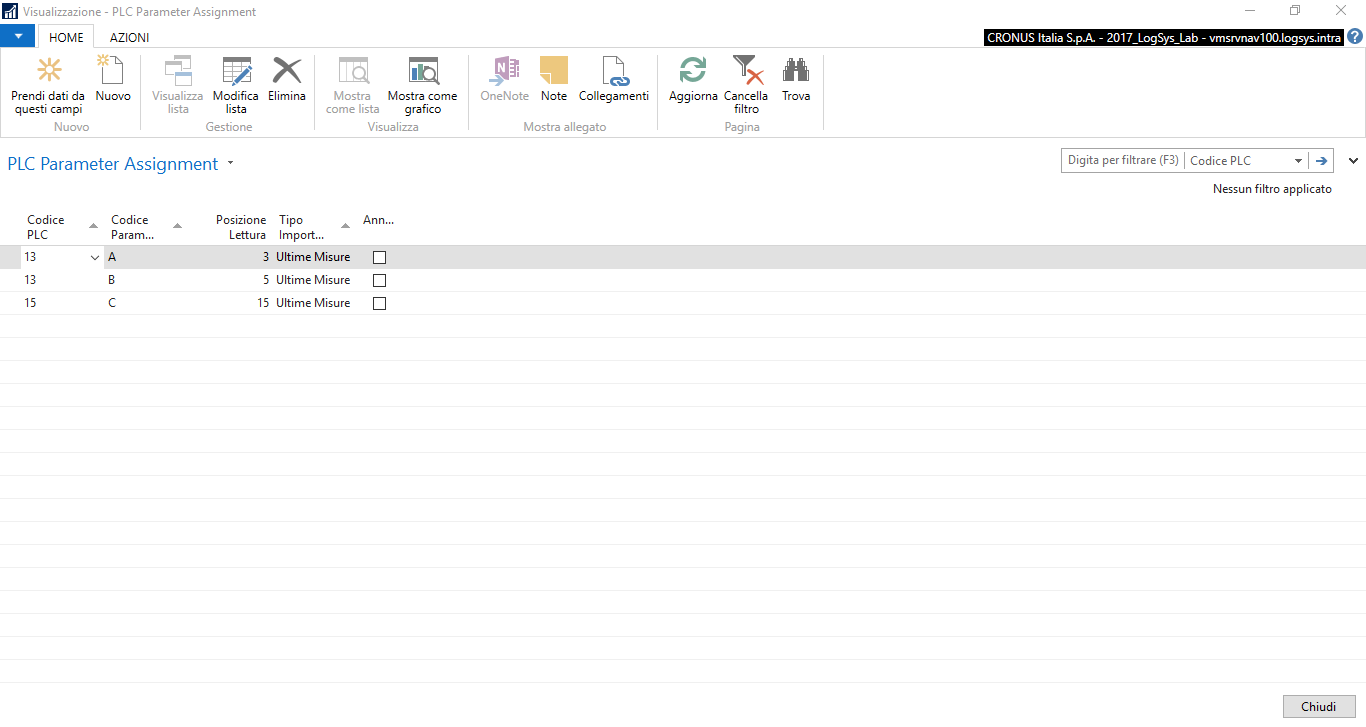
\includegraphics[width=1\textwidth]{images/PLCAssignmentList.png}
\end{frame}


\begin{frame}
\frametitle{Lista con i parametri}
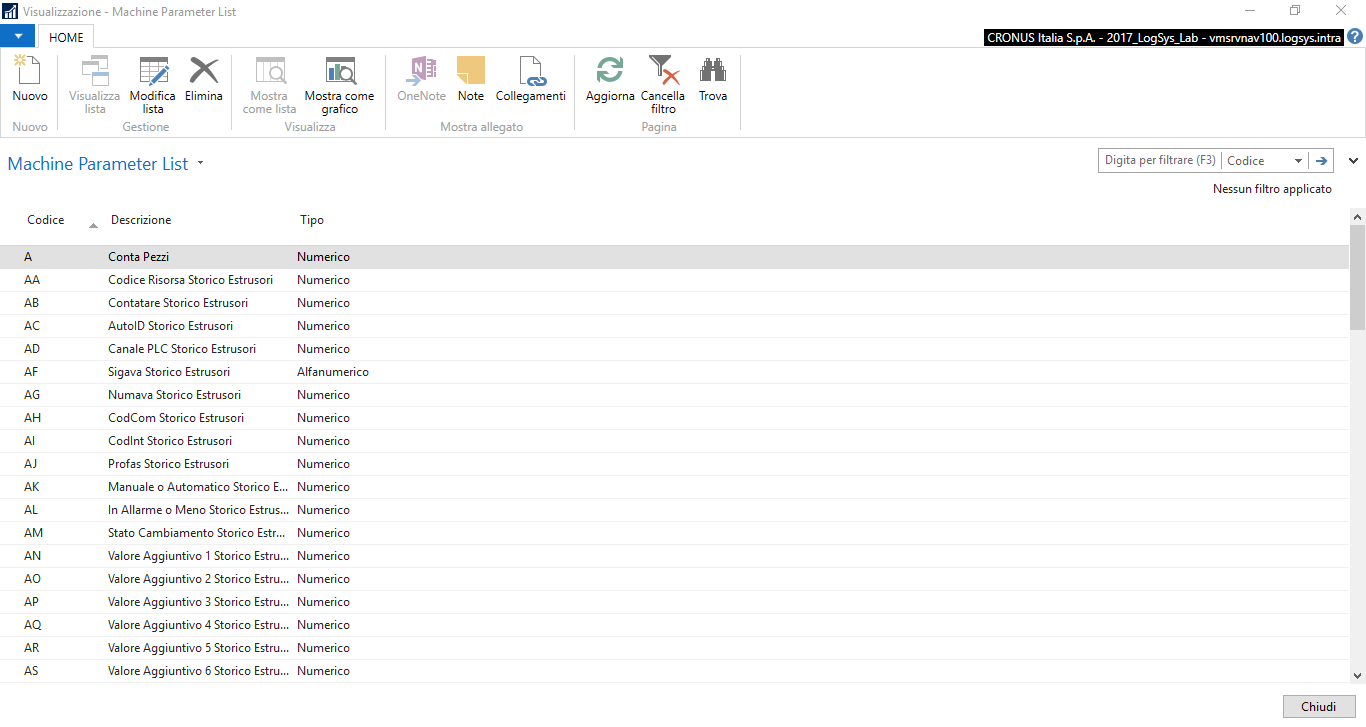
\includegraphics[width=1\textwidth]{images/MachineParameter.png}
\end{frame}

\begin{frame}
\frametitle{Pagina del token}
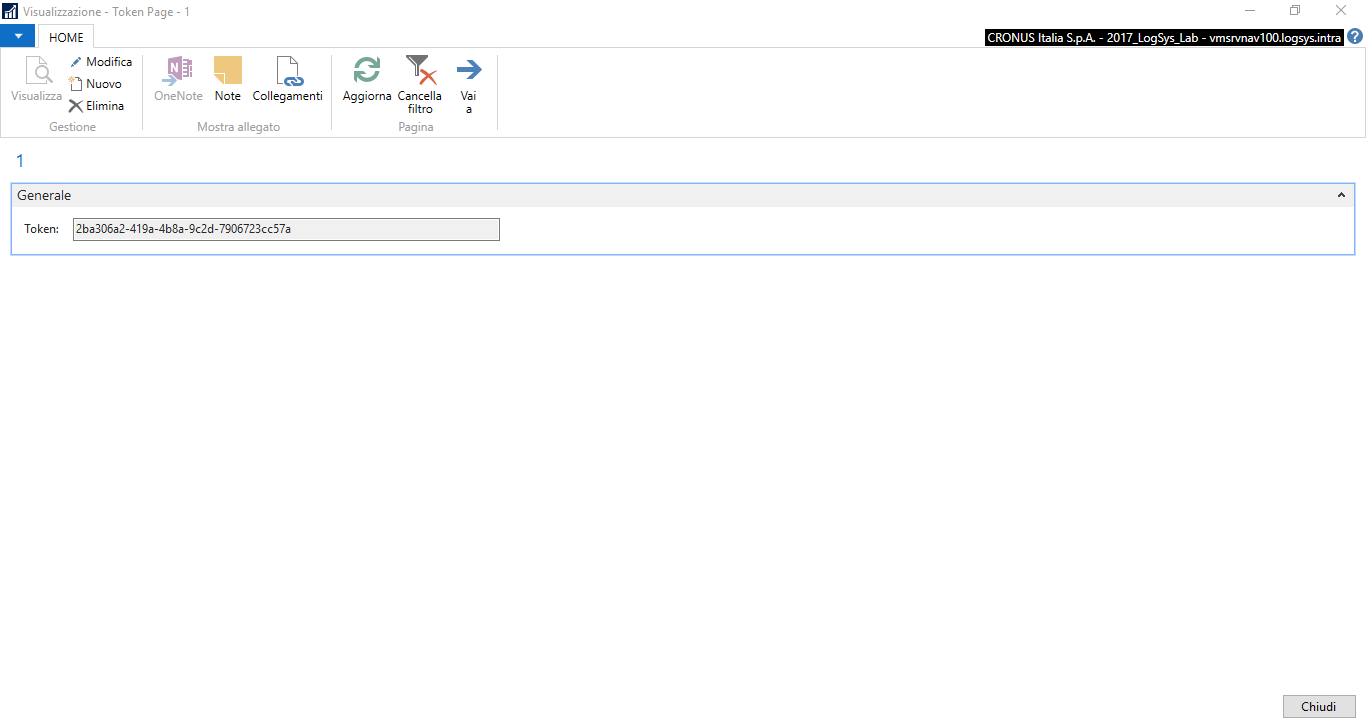
\includegraphics[width=1\textwidth]{images/tokenpage.png}
\end{frame}



\begin{frame}
\frametitle{PLC Reading List}
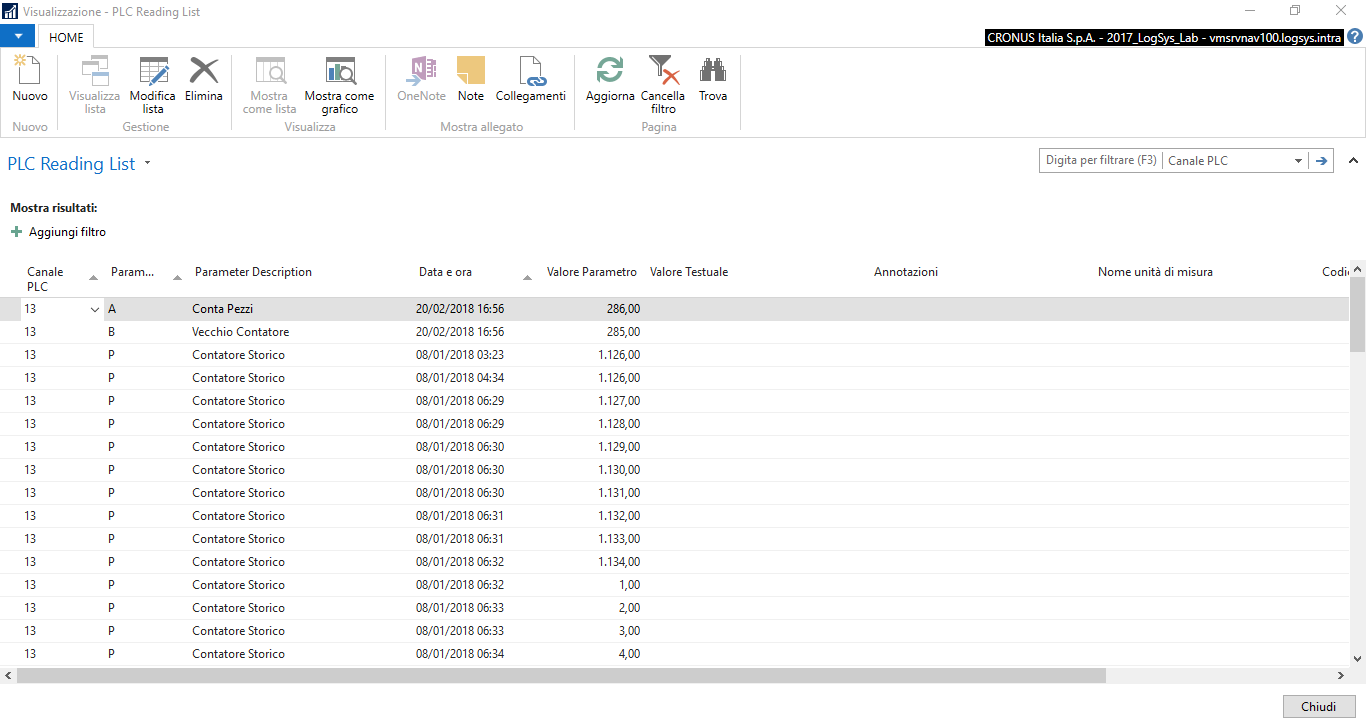
\includegraphics[width=1\textwidth]{images/PLCReadingList.png}
\end{frame}


\begin{frame}
\frametitle{Metodo SetMeasurementPLC}
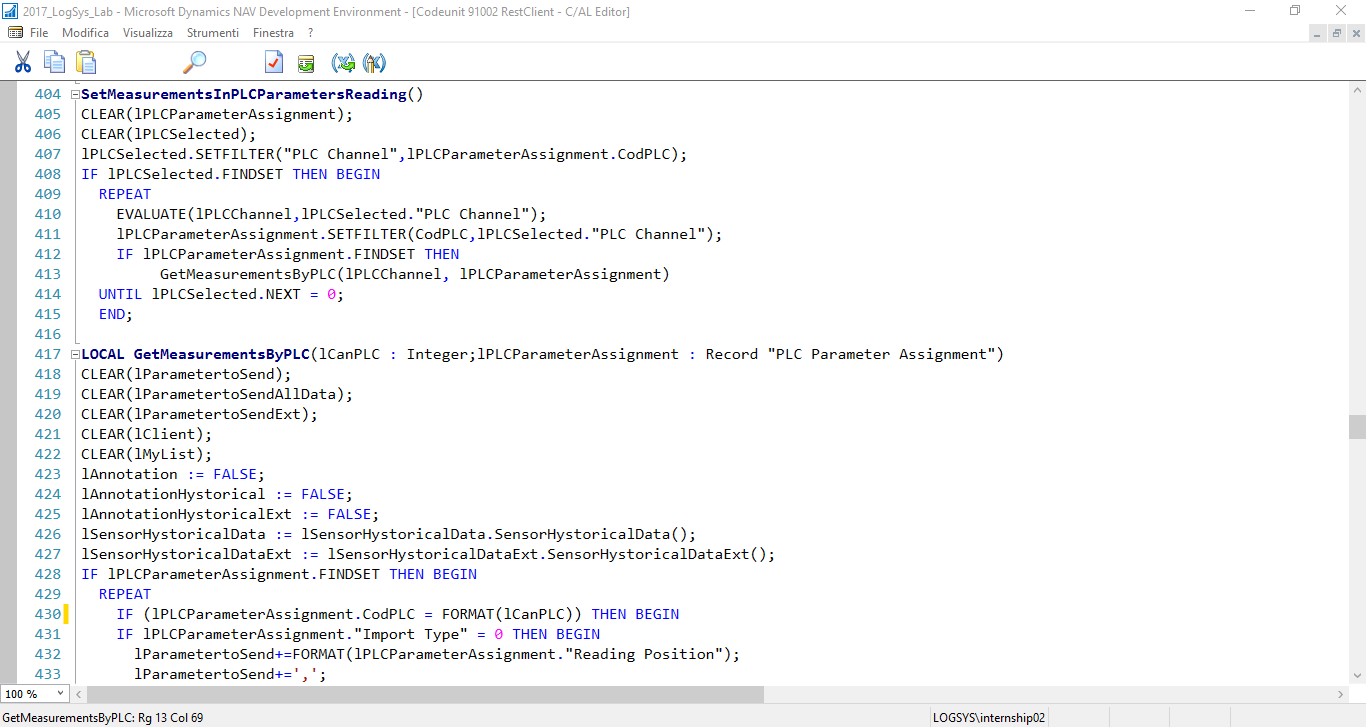
\includegraphics[width=1\textwidth]{images/NAVSetMesurament.png}
\end{frame}

\begin{frame}
\frametitle{Metodo GetMeasurementPLC1}
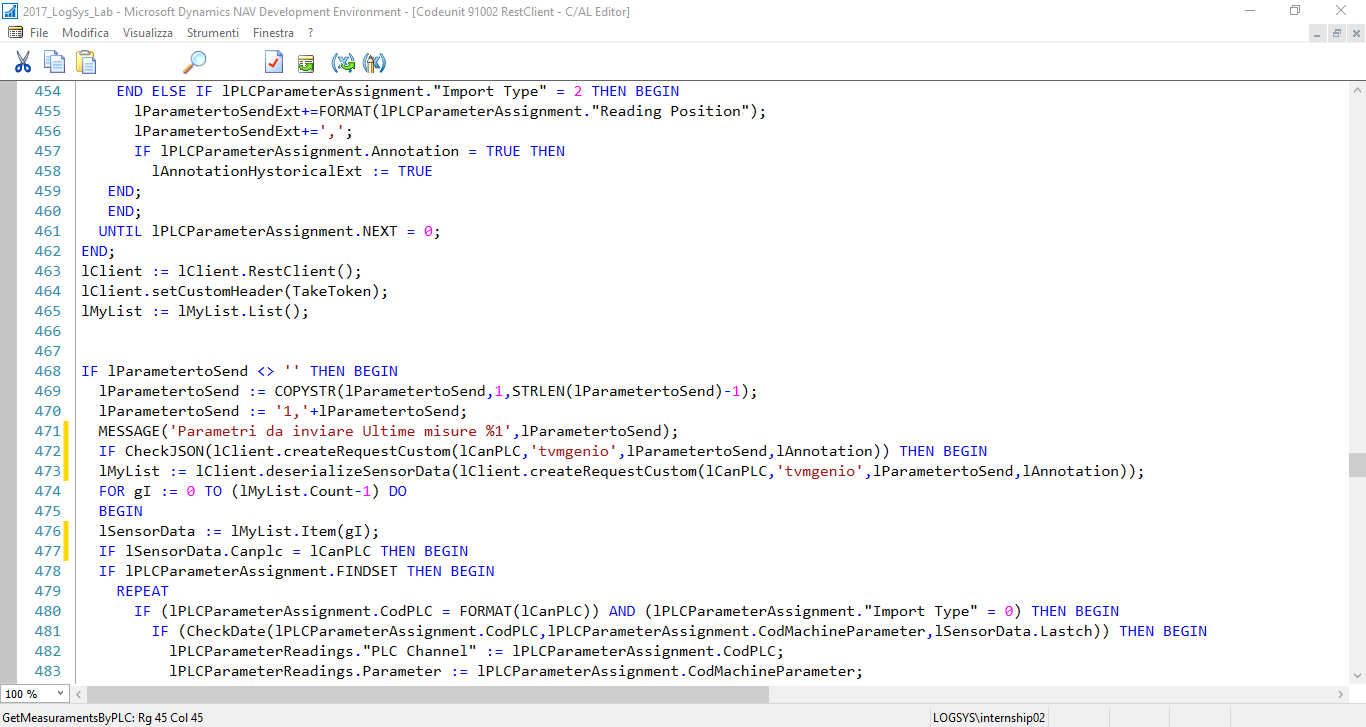
\includegraphics[width=1\textwidth]{images/NAVGetMesurament1.png}
\end{frame}

\begin{frame}
\frametitle{Metodo GetMeasurementPLC2}
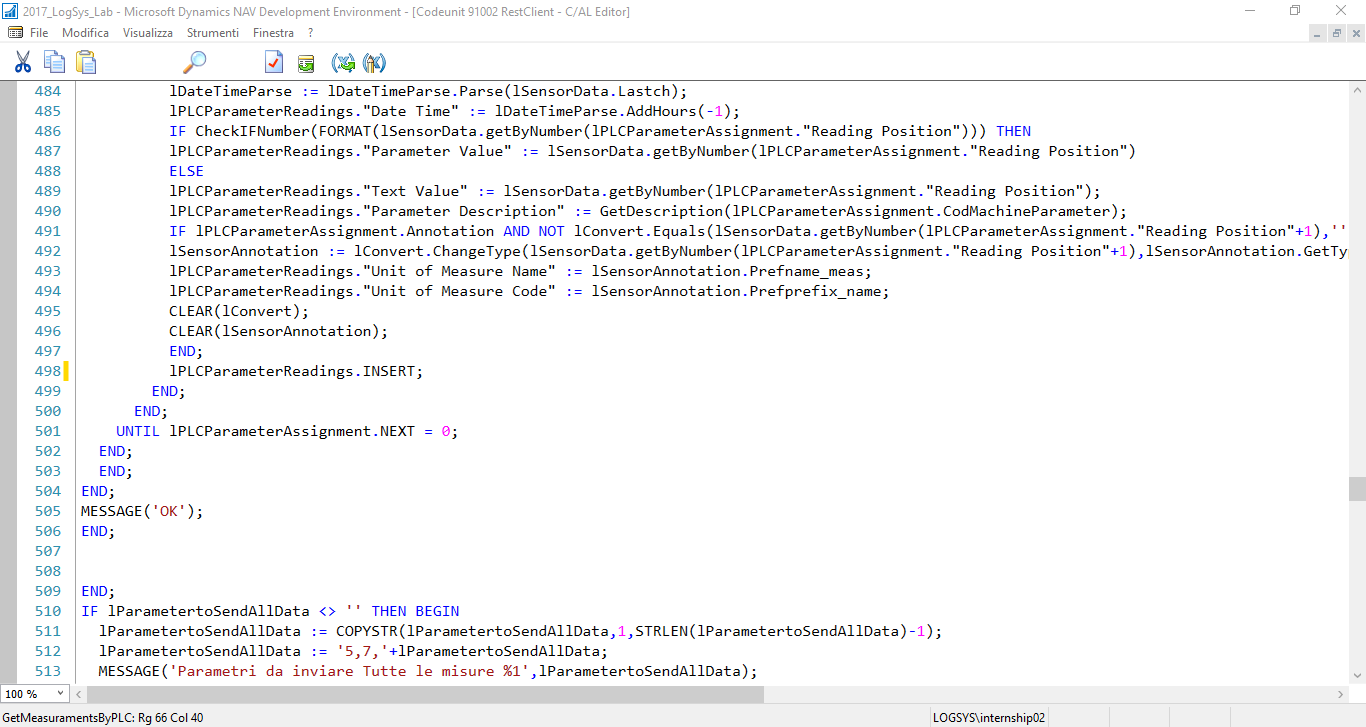
\includegraphics[width=1\textwidth]{images/NAVGetMesurament2.png}
\end{frame}

\begin{frame}
\frametitle{NAV servizi web}
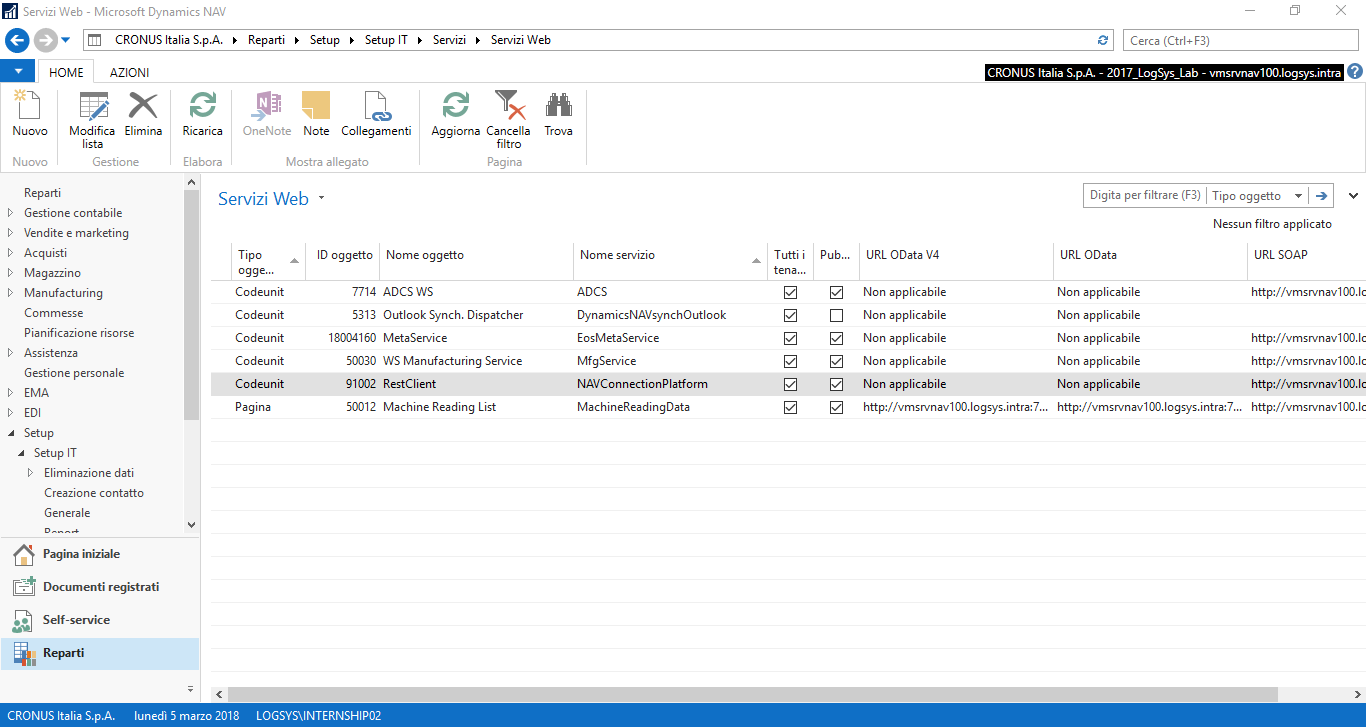
\includegraphics[width=1\textwidth]{images/NAVServiziWeb.png}
\end{frame}


\begin{frame}
\frametitle{NAV SubscriptionPage}
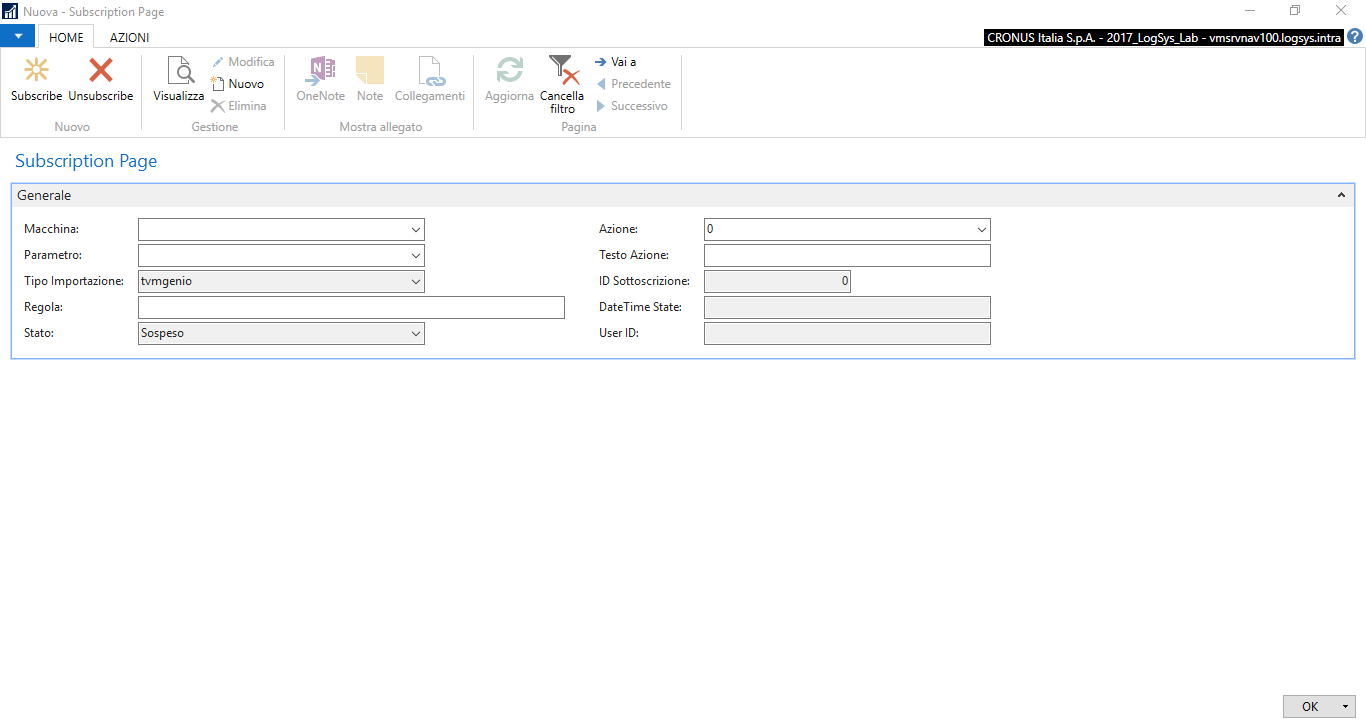
\includegraphics[width=1\textwidth]{images/NAVSubscriptionPage.png}
\end{frame}

\begin{frame}
\frametitle{Metodo PushMeasurement 1}
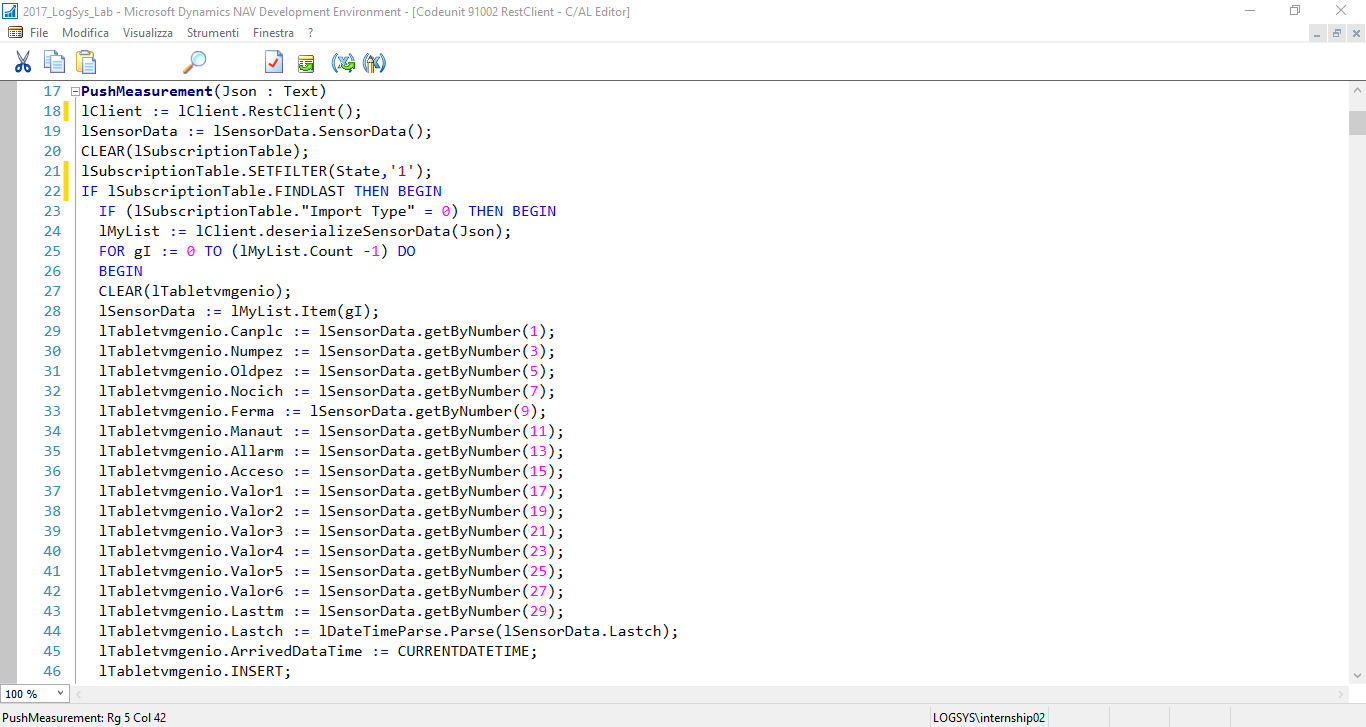
\includegraphics[width=1\textwidth]{images/NAVPushMeasuraments1.png}
\end{frame}

\begin{frame}
\frametitle{Metodo PushMeasurement 2}
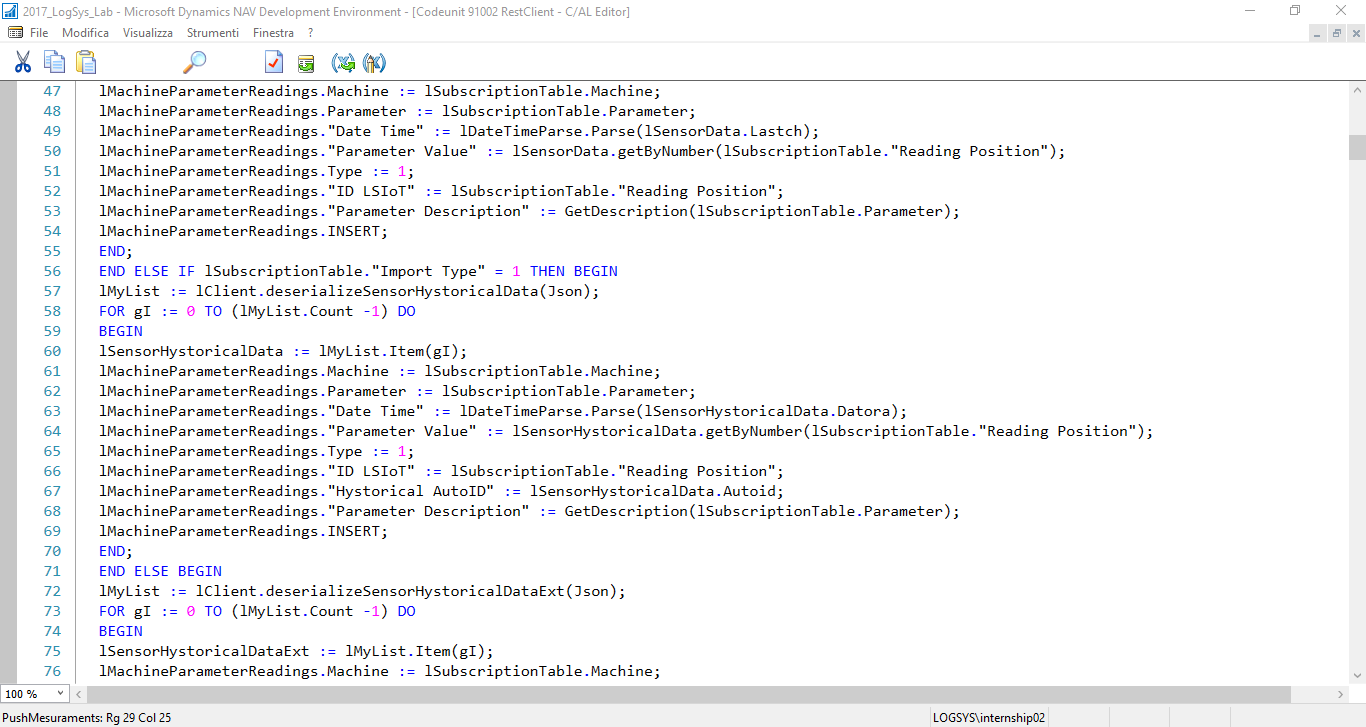
\includegraphics[width=1\textwidth]{images/NAVPushMeasuraments2.png}
\end{frame}

\begin{frame}
\frametitle{Metodo PushMeasurement 3}
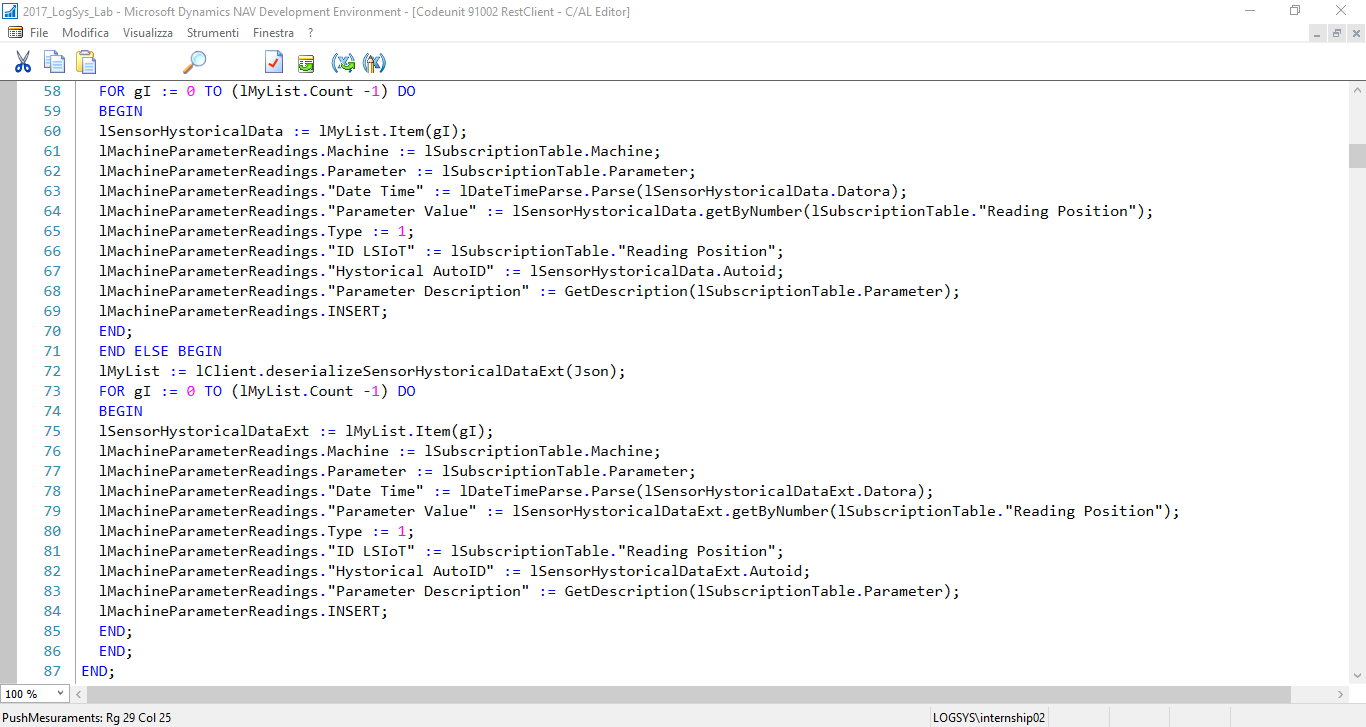
\includegraphics[width=1\textwidth]{images/NAVPushMeasuraments3.png}
\end{frame}

\end{document}